\section{Our Approach}

\begin{figure}
\begin{floatrow}
\centering

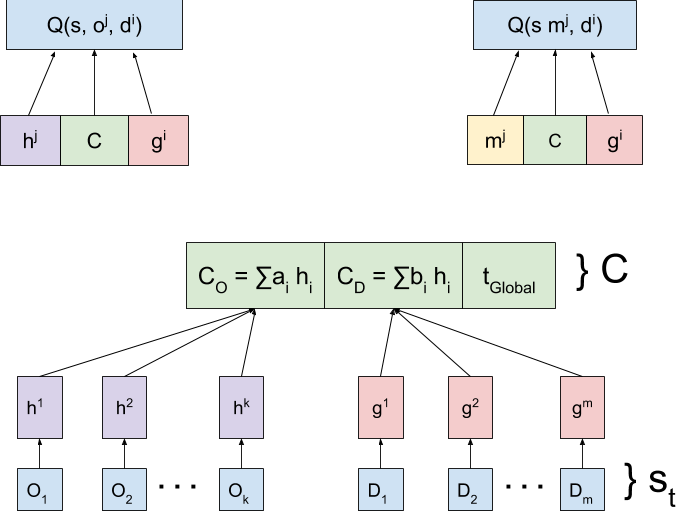
\includegraphics[width=.9\linewidth]{sections/mddqn/figures/Improved_Dispatch_Q-learning_2_.png}
\caption{The neural network architecture used in SD-DQN and MD-DQN. Order and driver embeddings are attended to for global context. The network then uses global context to query order/driver pairs (represented by the matrix in the top left) and reposition/driver pairs (represented by the matrix in the top right) to produce Q-values for all possible actions.}
\label{Figure:network}
\end{floatrow}
% \label{Figure:network}
\end{figure}

\subsection{Neural Network Overview}

At time $t$ there is a collection of orders $o_t^i \in \mathcal{O}_t$, drivers $d^j_t \in \mathcal{D}_t$, and subset $\mathcal{D}^{\mathrm{avail}}_t \subset \mathcal{D}_t$ of available drivers. A driver is available if it is not currently serving an order. State is given to the neural network as $s_t = (\mathcal{O}_t, \mathcal{D}_t, \mathcal{D}^{\mathrm{avail}}_t, t)$. At time $t$, the action space is made up of available driver-order pairings or non-repositioning driver-repositioning pairings.

\subsubsection{Input representation}
The exact vector representation of $o_t^i$ and $d_t^j$ depend on the environment. In the static assignment problem \cite{munkres1957algorithms}, we are only concerned with the position of drivers and {\em start positions} of orders. Therefore drivers and orders are each represented as two-dimensional vectors of their $x$ and $y$ coordinates. In MDVDRP, orders are given as six-dimensional vectors consisting of starting $x$ position, starting $y$ position, ending $x$ position, ending $y$ position, price, and time waiting, where time waiting is the difference between the current time and the time that the order first began requesting a driver. A driver is represented by a six-dimensional vector: an $x$ position, $y$ position, time to completion, repositioning x and y coordinates, and reposition counter. If the driver is available, its $x$ and $y$ position are given by its actual location, and time to completion is 0. If the driver is not available, the $x$ and $y$ position are the ending location of the order it is servicing, and the time to completion is the time it will take to finish the order. If a driver is repositioning, the direction of repositioning is reflected in the repositioning coordinates, and reposition counter counts down from the maximum repositioning time.

\subsubsection{Embedding and global context}
The network first embeds orders $\{o_t^i\}_i$ and drivers $\{d_t^j\}_j$ into memory cells $\{h_t^i\}_i$ and $\{g_t^j\}_j$ respectively found in the purple and red boxes in \cref{fig:network}. Then, a single round of attention is performed over each to produce a {\em global order context} $\mathcal{C}_t^O$ and {\em global driver context } $\mathcal{C}_t^D$. These contexts as well as global time are concatenated to produce a {\em global context vector} $\mathcal{C}_t^G$, which is the system's internal global representation of state.

\subsubsection{Action-value calculation}
The network then computes two types of Q-values: those for driver-order pairs and those for driver-reposition pairs. Each of these two processes can be viewed as their own attention mechanisms over pairs, with the attention coefficients interpreted as Q-values. More precisely, for available driver-order pairs we construct a small fully connected neural network $Att_o$ such that $Q(s_t, d_t^j, o_t^i) = Att_o(C_t, g_t^j, h_t^i)$. Similarly, for available driver-reposition pairs, we construct another small neural network $Att_r$, so that $Q(s_t, d_t^j, m_t^i) = Att_r(C_t, g_t^j, m_t^i)$ where $m_t^i$ is a vector representation of a reposition action. The top left of \cref{fig:network} represents a generic example of $Att_o$ while the top right represents $Att_r$. In all repositioning experiments, there are 9 reposition actions consisting of 8 cardinal directions and a stationary action (no movement). The $m_t^i$'s are represented as one-hot vectors, and displayed as yellow boxes in \cref{Figure:network}. 

\subsection{Single-driver and multi-driver Q-values}

% \begin{figure}
% \begin{floatrow}
% \centering
% 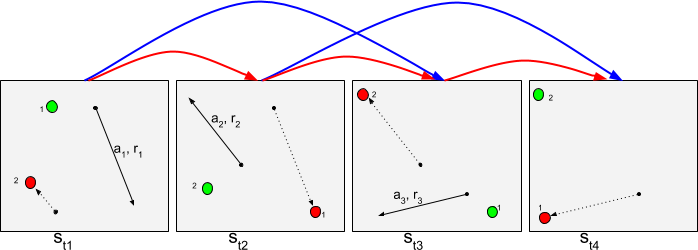
\includegraphics[width=1.\linewidth]{dqn_state_transitions_cropped.png}\label{fig:dqn_trans}
% \caption{The above image shows a length 4 trajectory. The currently available driver is green, dispatched driver is red, and the order that the available driver accepts at time $t_i$ is $a_i$ and has price $r_i$. The accepted order at time $t_i$ is labeled by its action name and price, $(a_i, r_i)$ and travels from the solid black dot to the terminal arrow. SD-DQN transitions are indicated by blue arrows above state, e.g. transition $(s_{t1}, a_1, r_1, s_{t3})$, which is driver-centric with respect to driver 1. MD-DQN transitions are indicated by red arrows e.g. transition$(s_{t1}, a_1, r_1, s_{t2})$, which transitions from a state where driver 1 is available to a state where driver 2 is available.}
% \end{floatrow}
% \end{figure}

We take two approaches to training the above network: single-driver DQN (SD-DQN) and multi-driver DQN (MD-DQN). Each can be viewed as a 1-step bootstrapping approach like in the standard DQN, but they differ from one another in the form of one step data that is given to the network. As a result, the learned $Q$-values in each approach have distinct semantics.

In SD-DQN, we use {\em driver-centric} transitions. At time $t$, the system is in global state $s_t = (\mathcal{O}_t, \mathcal{D}_t, \mathcal{D}^{avail}_t, t)$ and a driver-order or driver-reposition action is selected, yielding reward $r_t$. Let $d$ be the selected driver, and $a_t$ denote the action. We then proceed to make dispatching and repositioning decisions for other drivers as they become available, until eventually driver $d$ is available again in state $s_{t'} = (\mathcal{O}_{t'}, \mathcal{D}_{t'}, \mathcal{D}^{avail}_{t'}, t')$. The change in time $t'-t$ is the time it takes for driver $d$ to complete a single trip or repositioning, which is typically between $10$ and $30$ minutes for trips or $2-3$ minutes for repositionings. In SD-DQN, this yields a transition $(s_t, a_t, r_t, s_{t'})$. To train our network in the SD-DQN setting, we update the outputs of the network using the target:
% * <xiaocheng.t@gmail.com> 2018-08-14T21:26:15.259Z:
% 
% o_t^i or o_i^t
% John: FIXED
% ^.

\begin{equation}
% * <xiaocheng.t@gmail.com> 2018-08-14T21:18:28.781Z:
% 
% here the max is over all orders in t'. The notation should be $O_{t'}$ right?
% 
% ^.
\widehat{Q}(s_t, a_t; \theta_t) = r_t + \gamma^{t' - t} \cdot \max_{a'} Q^T(s_{t'}, a'; \theta_t'),
\end{equation}
where $\theta_t$ are the current network weights and $\theta_t'$ are the weights of the target network, which are slow updating weights that sync with the network's current weights at fixed intervals. To account for the fact that transitions occur over a variable time interval, future value is discounted continuously with discount factor $\gamma$. The network is trained to reduce the Huber loss between $\widehat{Q}(s_t, a_t)$ and $Q(s_t, a_t)$. Intuitively, SD-DQN updates the network towards driver-centric Q-values, only accounting for the discounted return associated to a single driver. We collect driver-centric transitions from each driver into a single shared replay buffer. The drawback of this method is that, as we learn the single driver Q-values, we update the behavior of {\em all drivers}, and so one perspective is that the driver, as an agent, is learning in a nonstationary MDP. This has the potential to cause instability issues in training, though we did not observe such issues in our experiments. Another issue with SD-DQN is that it may train single drivers to behave selfishly. That is, drivers might learn to choose actions that are best for themselves rather than actions that promote the greatest overall reward for the system. This issue is raised in work on learning in collectives \cite{wolpert2002optimal,tumer2004time}, however the interaction of individual learning and system optimization is not well understood.
% * <xiaocheng.t@gmail.com> 2018-08-14T21:27:02.543Z:
% 
% o_t^i or o_i^t
% John: FIXED
% ^.

In MD-DQN we use {\em system-centric} transitions. At time $t$, the system is in global state $s_t = (\mathcal{O}_t, \mathcal{D}_t, \mathcal{D}^{\mathrm{avail}}_t, t)$ and we select action $a_t$, yielding reward $r_t$. When the next new driver becomes available, we transition to state $s_{t'} = (\mathcal{O}_{t'}, \mathcal{D}_{t'}, \mathcal{D}^{\mathrm{avail}}_{t'}, t')$. In contrast to the SD-DQN transition, the change in time $t'-t$ is the time it takes for the next available driver to appear, which is on the order of fractions of a second in large cities. As in the SD-DQN case, this yields a 1-step transition $(s_t, a_t, r_t, s_{t'})$. We use the same target and update procedure from equation (1), but with this different transition as input data. MD-DQN will update the network towards a global, system-centric Q-value that sums the discounted rewards of all drivers together. This means the Q-values produced by MD-DQN will be approximately $n$ times larger than those of SD-DQN, where $n$ is the number of drivers. Ignoring issues related to function approximation MD-DQN provides a correct learning signal for solving an MDVDRP. However, as a practical matter, the Q-values learned in MD-DQN are based on many more transitions, and therefore should be harder to learn. This has been our empirical experience. In the results section we describe steps we needed to take in order to stabilize MD-DQN learning, but the primary change we make is to do $n$-step Q-learning \cite{mnih2016asynchronous} with $n$ equal to the number of drivers in the system.
% * <xiaocheng.t@gmail.com> 2018-08-14T21:36:01.530Z:
% 
% >  this yields a transition $(s_t, o_i^t, r_t, s_{t'})$
% o_t^i or o_i^t
% John: FIXED
% ^.
% * <xiaocheng.t@gmail.com> 2018-08-14T21:28:28.742Z:
% 
% > When the next driver becomes available
% when multiple drivers become available I assume we randomly pick one to compute the target value? Will the target value differ a lot given different driver we pick? 
% 
% ^.
% * <xiaocheng.t@gmail.com> 2018-08-14T21:27:26.269Z:
% 
% o_t^i or o_i^t
% John: FIXED
% ^ <xiaocheng.t@gmail.com> 2018-08-14T21:34:41.241Z.


\subsection{Architecture details}

For ease of exposition, in the following section we omit subscript $t$'s that had denoted time in previous sections.

{\bf Memory embedding.} We begin with a global state $s$, consisting of order and drivers and time. All orders and drivers are both embedded into length 128 memory cells using a single layer network with 128 output units followed by RELU nonlinearities. 

{\bf Attention for global context.} Given a set of $N$ order memories $h^i$ and $M$ driver memories $g^j$. The attention mechanism for orders/drivers are given by the following equations:
\begin{align*}
C^O = \sum_{i=1}^{N} a_i h^i \\
\\
C^D = \sum_{j=1}^{M} b_j g^j
\end{align*}

\noindent where
\begin{equation}
a_i = \sigma(v_o \cdot \mathrm{tanh}(W^O \cdot h^i)), 
b_j = \sigma(v_d \cdot \mathrm{tanh}(W^D \cdot g^j))
\end{equation}

\noindent and $\sigma$ is a sigmoid activation function, $W^O$ and $W^D$ are 128 dimensional square matrices, and $v^O$ and $v^D$ are 128 dimensional vectors so that $a_i$ and $b_j$ are scalars. Both W's and v's are trained. \newline
% * <xiaocheng.t@gmail.com> 2018-08-14T00:31:00.726Z:
% 
% Here is $W^O$ the same as $W_o$?
% Answer: Yes, also with W^D and W_d. I changed it so notation is consistent
% ^.

We concatenate the two contexts, along with the episode time $t$, to produce a 257 dimensional global context vector

\begin{equation}
C_G = [C_o | C_d | t],
\end{equation}

{\bf Q-values.} To compute a driver-order Q-value $Q(s, d^j, o^i)$, we concatenate the global context with the order's memory embedding $h^i$ and driver's memory embedding $g^j$, and pass this through a fully connected layer with 64 units and RELU activation, and finally pass this to a single linear unit. We use the same network architecture for driver-repositioning pairs, but we {\em do not} share weights between the driver-order network and driver-repositioning network.

\subsubsection{Further training details}

In all experiments, we use a replay memory that is initialized with random behavior transitions. The size of replay memory as well as how frequently the target network is synced are both environment dependent, and are specified in the appendix. We also use a target network for setting Q-value targets. During training, each training loop begins by taking one step in the environment. Behavior is $\epsilon$-greedy with respect to the network's Q-values, where $\epsilon$ is linearly annealed in all experiments as specified in the appendix. For both SD-DQN and MD-DQN, one new transition will be added to replay memory (though they differ in what this one step transition is). Then, we sample a batch of 32 transitions from replay memory, and perform a Q-value update using equation (1). For all experiments, $\gamma = 0.99$. Gradients are applied using the Tensorflow implementation of RMSProp with gradients clipped at 100.
